\section{Experiment=26: Plume-lithosphere interaction a la Wang \& Li (2021)}

The setup is based on \fullcite{wali21}. 

The recipe is as follows: CitcomCU, Boussinesq approximation, 3d, resolution 256x256x96,
angular opening is $90^o$ in both directions, standard values for mantle
physical parameters.
The rheology is of the Frank-Kamenetskii type: $\eta^\star=\exp (E^\star(1-T^\star))$ 
where the starred quantities are dimensionless. 

The parameters are as follows:
\begin{lstlisting}
Rsurf = 6370e3
Rcmb = Rsurf - 1000e3
rho0 = 3300
g = 9.8
eta0 = 1e21
R = 8.314
alpha = 3e-5
kappa = 1e-6
hcapa = 1250
hprod=4e-12 # W/kg
Tsurf = 273
DeltaT = 1350
year = 365.25 * 24 * 3600
\end{lstlisting}

The dimensionless temperature is 0 at the top and 1 at the bottom, while
the real temperature difference is stated to be 1350C. We then dedude that
\[
T^\star = \frac{T-T_K}{\Delta T}
\]
where $T_K=273$. We then have $T_{top}=273$ and $T_{bottom}=1350C=1623K$.

The dimensionless viscosity is temperature-dependent and simply given by
$\eta^\star(T^\star)=\exp (E(1-T^\star))$ with $E=6.91$.
We then have
\[
\eta(T) 
= \eta_0 \exp \left[ E \left(1 - \frac{T-T_K}{\Delta T} \right)  \right]
\]
See stone 183 for profiles.

The temperature boundary condition at the bottom is $T_{bottom}=1350$
and the temperature anomaly of the plume exponentially decreases from plume
centre to plume edge
by $\Delta T = \Delta p_T \exp (-r^2/R_p^2)$
where $R_p$ and $\Delta T_p$
are the radius and excess temperature of the plume, respectively, and
$r$ is the distance from the plume centre.
In the reference case the authors use $R_p=300km$, $\Delta T_p=300$.

The initial temperature is not entirely clear. I then settle for a half-space 
cooling model at the surface with an age of 80 Ma and a mantle temperature
equal to the bottom value.

\begin{center}
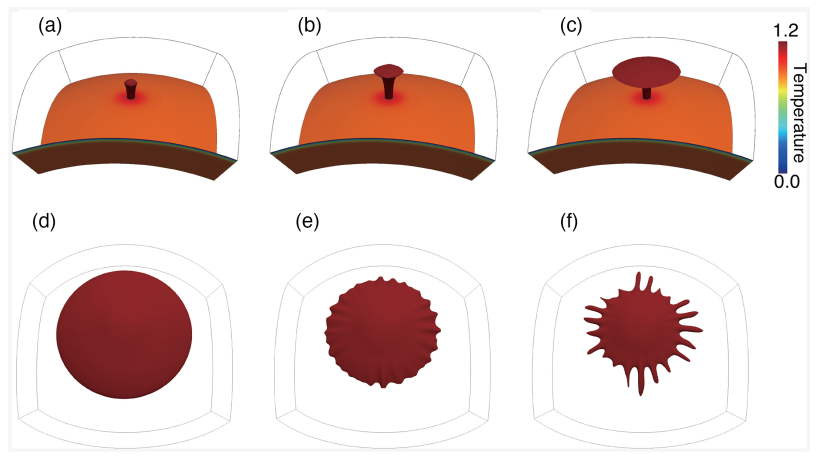
\includegraphics[width=10cm]{exp26/wali21}
\end{center}

In this case we run the model in 2d only.


\begin{center}
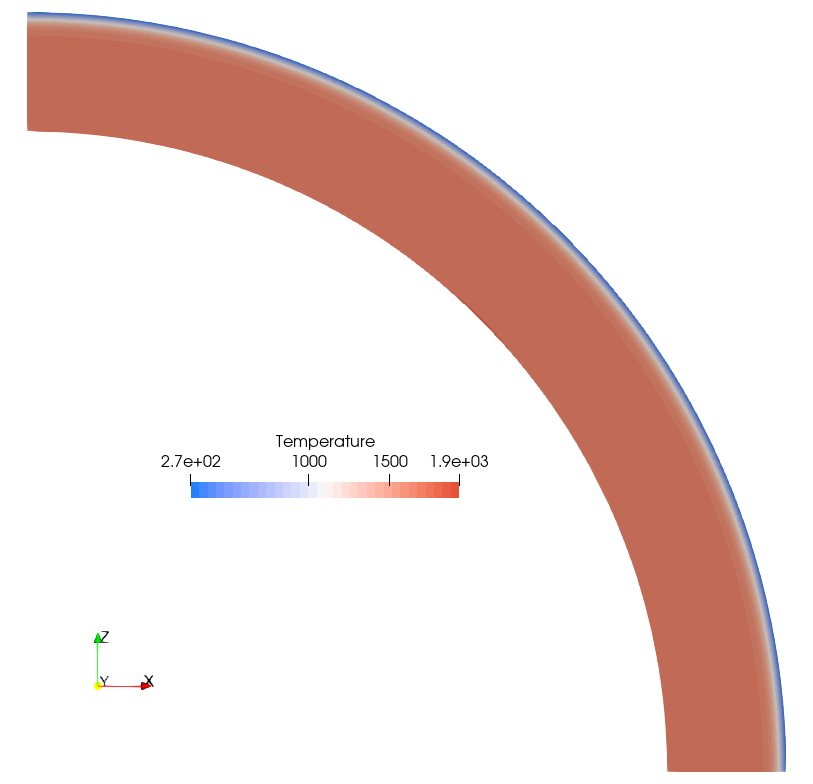
\includegraphics[width=4cm]{exp26/T.0000.png}

\includegraphics[width=4cm]{exp26/eta.0000.png}\\
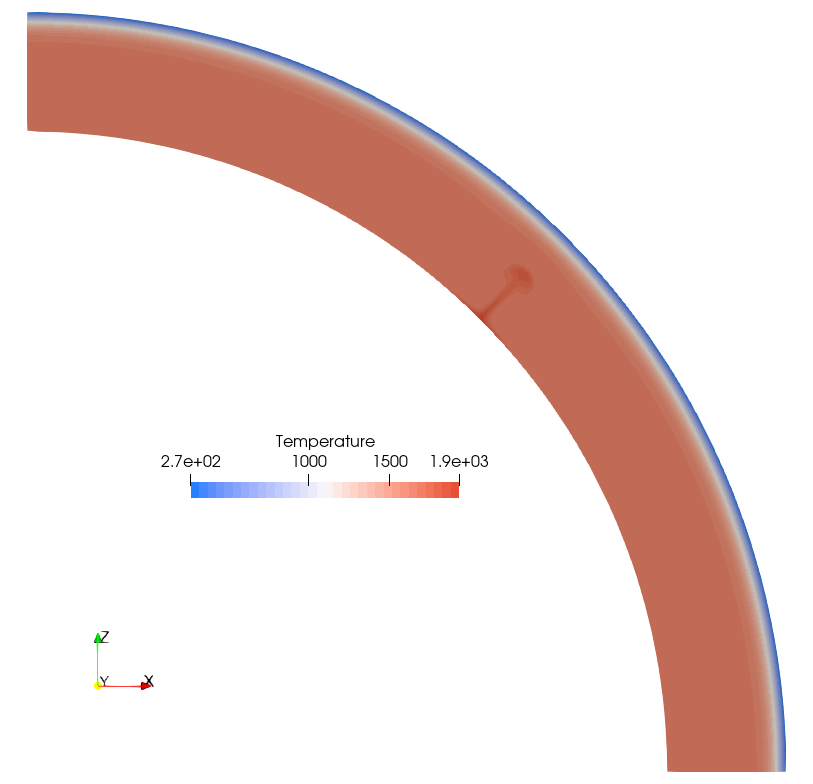
\includegraphics[width=4cm]{exp26/T.0015.png}
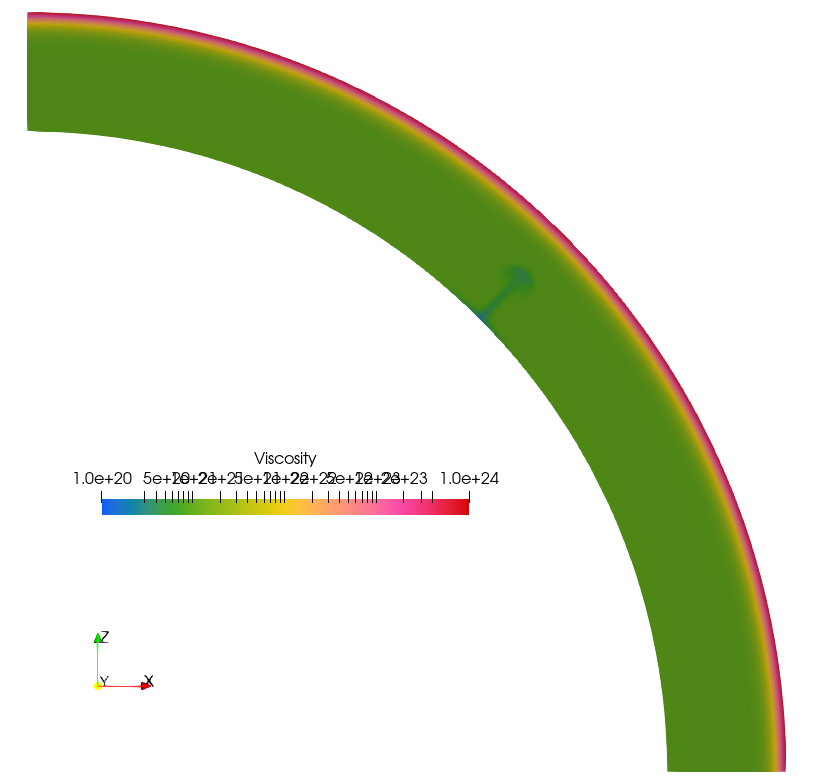
\includegraphics[width=4cm]{exp26/eta.0015.png}\\
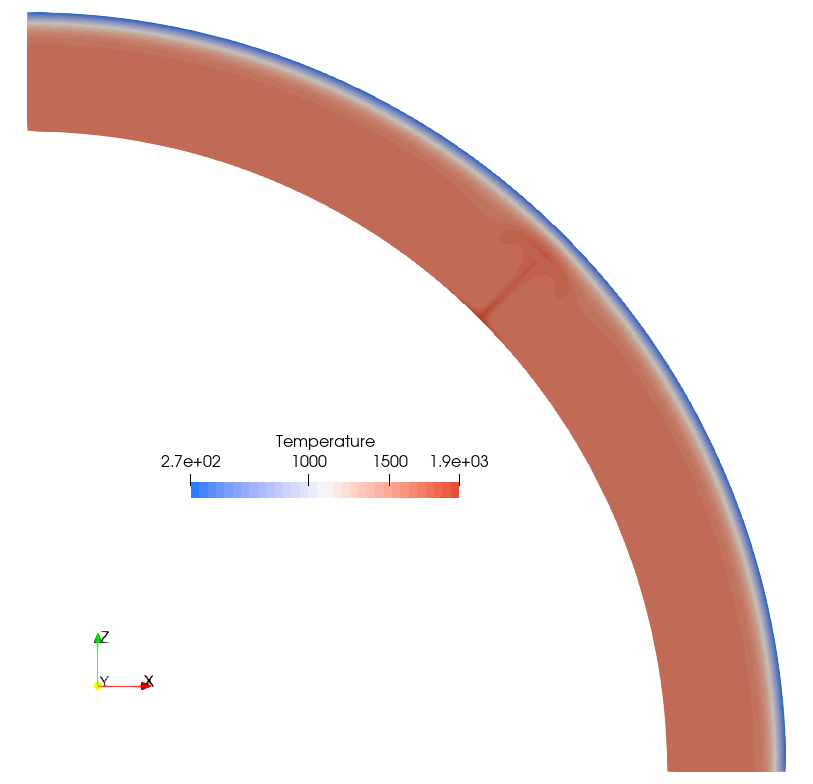
\includegraphics[width=4cm]{exp26/T.0030.png}
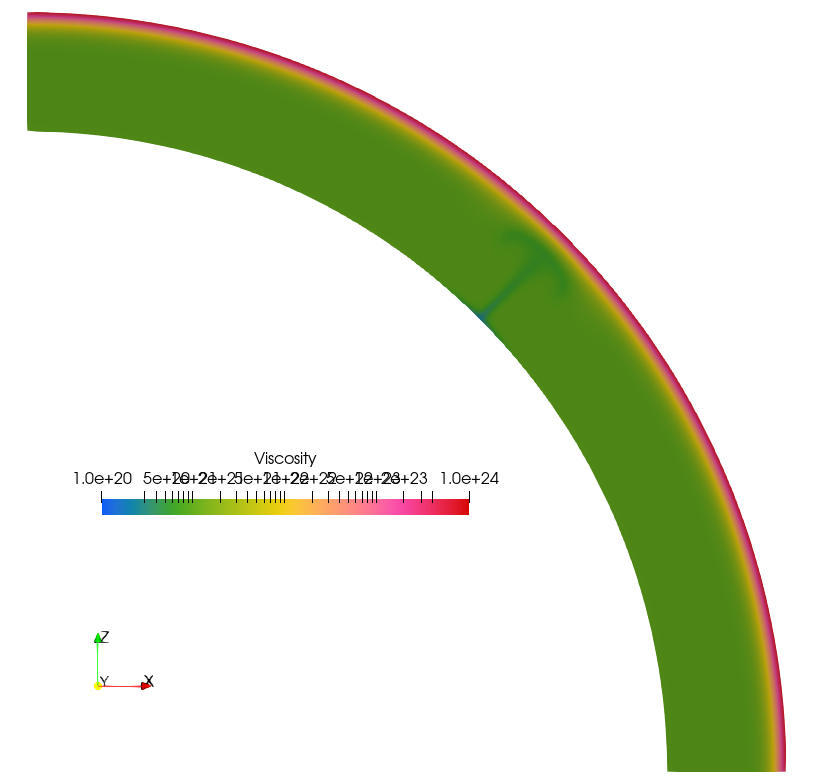
\includegraphics[width=4cm]{exp26/eta.0030.png}\\
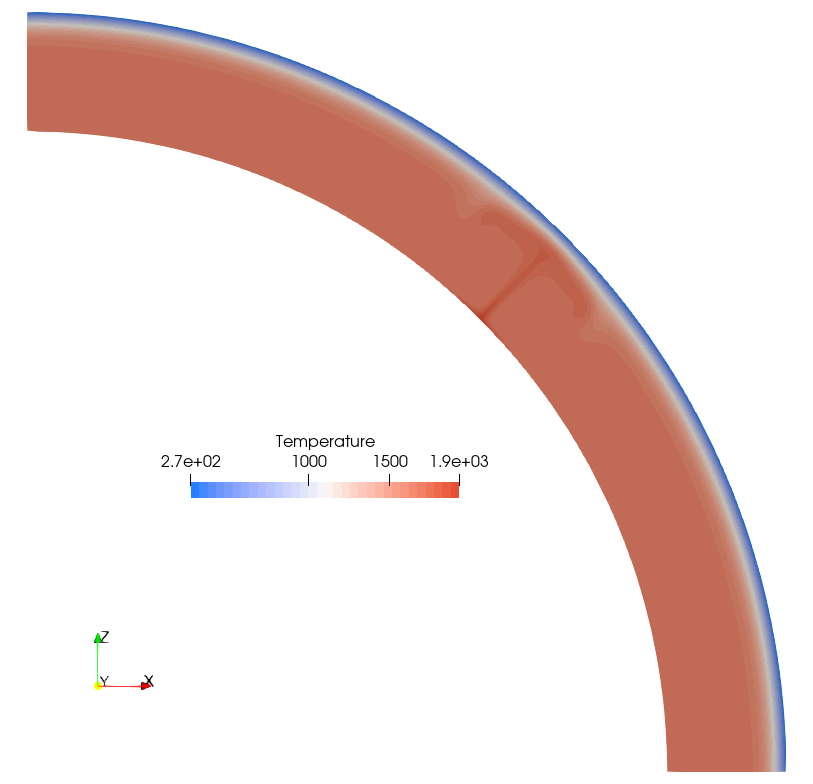
\includegraphics[width=4cm]{exp26/T.0045.png}
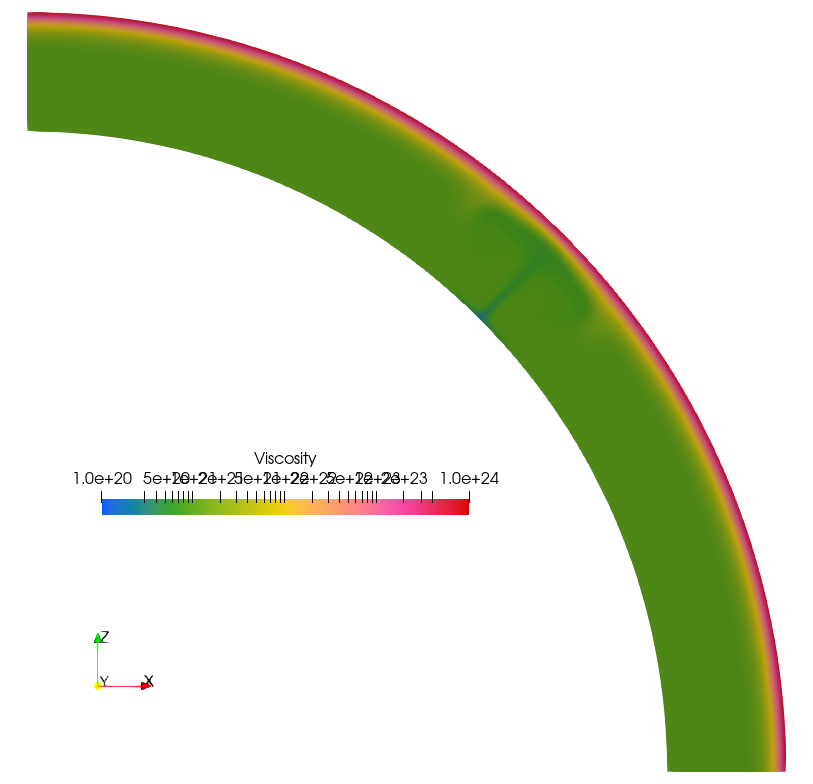
\includegraphics[width=4cm]{exp26/eta.0045.png}\\
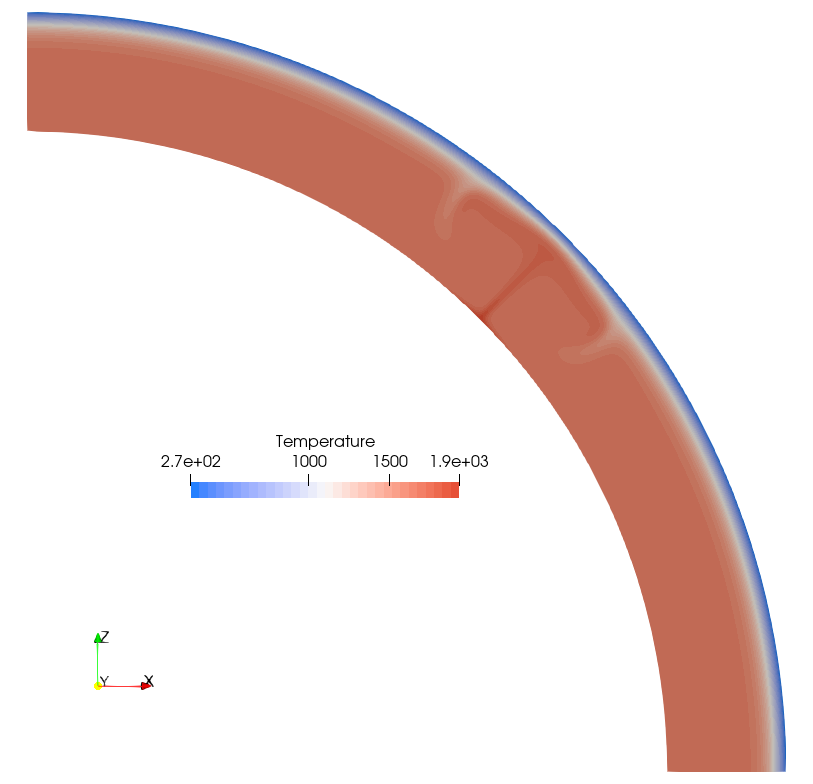
\includegraphics[width=4cm]{exp26/T.0060.png}
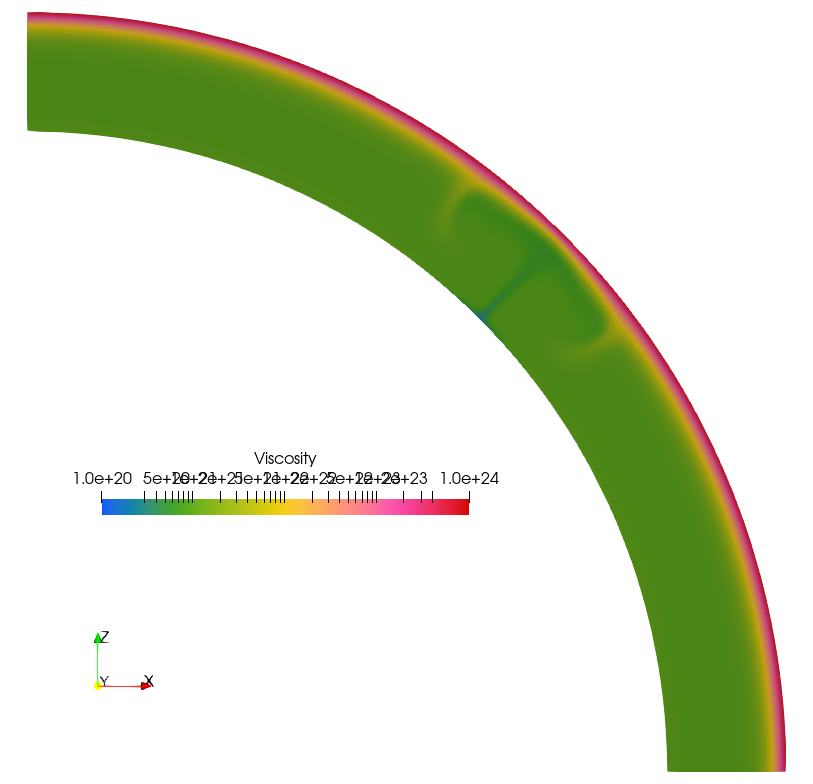
\includegraphics[width=4cm]{exp26/eta.0060.png}\\
Obtained with nelz=48.
\end{center}



 
